\documentclass{standalone}
\usepackage{tikz}

\usetikzlibrary{math}


\begin{document}

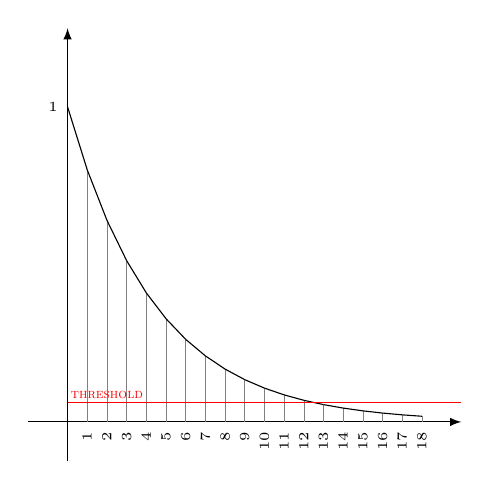
\begin{tikzpicture}
  \draw[-latex] (-0.5,0) -- (5,0);
  \draw[-latex] (0,-0.5) -- (0,5);

  \foreach[count=\i,remember=\y as \lasty (initially 4),remember=\x as \lastx (initially 0)] \x in {0.25,0.5,...,4.5} {
    \tikzmath{
      real \y;
      \y = 4 * 0.8^(4 * \x);
    }
    \draw[help lines] (\x,\y) -- (\x,0);
    \node[anchor=east,font=\tiny,rotate=90] at (\x,0) {$\i$};
    \draw (\lastx,\lasty) -- (\x,\y);
  }

  \draw[red] (0,0.25) -- (5,0.25) node[at start,anchor=south west,font=\tiny\sc,inner sep=1pt] {threshold};

  \node[anchor=east,font=\tiny] at (0,4) {$1$};
\end{tikzpicture}

\end{document}